\section{Task 1}

\href{https://github.com/lvjonok/f22-theoretical-mechanics/blob/master/homework3/task1.ipynb}{Source code}

\href{https://lvjonok.github.io/f22-theoretical-mechanics/2022/09/18/homework3.html}{Simulations}

\begin{enumerate}
    \item I assume point $M$ moves from A to B,
          so I actually have not $OM$, but rather $AO$ in motion equation.
    \item Find derivatives of motion and angle equations: \\
          Equation of motion:
          \begin{align}
              s_r(t) = 6 \pi t^2      \\
              \dot{s_r}(t) = 12 \pi t \\
              \ddot{s_r}(t) = 12 \pi
          \end{align}
          Equation of rotation:
          \begin{align}
              \phi(t) = \pi t^3/6       \\
              \dot{\phi}(t) = \pi t^2/2 \\
              \ddot{\phi}(t) = \pi t
          \end{align}
    \item Obtain positions of all points:
          \begin{enumerate}
              \item Position of point $O_1$:
                    \begin{answer}
                        \begin{align}
                            \vec{r}_{O_1}(t) = \begin{bmatrix}
                                0 \\
                                0
                            \end{bmatrix}
                        \end{align}
                    \end{answer}
              \item Position of point $O_2$:
                    \begin{answer}
                        \begin{align}
                            \vec{r}_{O_2}(t) = \begin{bmatrix}
                                2 \cdot R \\
                                0
                            \end{bmatrix}
                        \end{align}
                    \end{answer}
              \item Position of point $O$. It rotates around $O_1$:
                    \begin{answer}
                        \begin{align}
                            \vec{r}_{O}(t) = \begin{bmatrix}
                                \cos(\phi(t)) \\
                                \sin(\phi(t))
                            \end{bmatrix}
                        \end{align}
                    \end{answer}
              \item Position of point $A$. It rotates around $O_2$:
                    \begin{answer}
                        \begin{align}
                            \vec{r}_{A}(t) = \begin{bmatrix}
                                2 \cdot R + R \cdot \cos(\phi(t)) \\
                                R \cdot \sin(\phi(t))
                            \end{bmatrix}
                        \end{align}
                    \end{answer}
              \item Position of point $M$. It follow semicircle from $A$ to $O$.
                    Using $s_r(t)$ we can find an angle $\theta$ for $M$ as angle inside object $D$.\\
                    \begin{center}
                        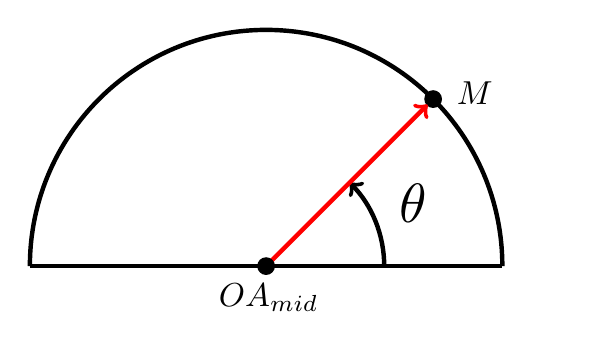
\begin{tikzpicture}
                            \draw[ultra thick] (0, 0) arc (180:0:3);
                            \draw[ultra thick] (0, 0) -- (6, 0);
                            \filldraw ({3 + 3 * cos(45)}, {3 * sin(45)}) circle (3pt);
                            \draw[ultra thick,->] (4.5, 0) arc (0:45:1.5);
                            \node[text width=1cm, scale=2] at (5.7, 0.8) {$\theta$};
                            \draw[red, ultra thick,->] (3, 0) -> ({3 + 2.9 * cos(45)}, {2.9 * sin(45)});
                            \filldraw (3,0) circle (3pt);
                            \node[text width=1cm, scale=1.2] at (3, -0.4) {$OA_{mid}$};
                            \node[text width=1cm, scale=1.2] at ({3.9 + 3 * cos(45)}, {3.1 * sin(45)}) {$M$};
                        \end{tikzpicture}
                    \end{center}

                    \begin{answer}
                        \begin{align}
                            \theta(t) = s_r(t) / R = 6 \pi t^2 / R \\
                            \vec{r}_{M}(t) = \frac{\vec{r}_{O}(t) + \vec{r}_{A}(t)}{2} + R \cdot \begin{bmatrix}
                                \cos(\theta(t)) \\
                                \sin(\theta(t))
                            \end{bmatrix}
                        \end{align}
                    \end{answer}
          \end{enumerate}

    \item Find velocities for $M$
          \begin{enumerate}
              \item Relative velocity. We consider motion of $M$ relative to $OA_{mid}$.
                    \begin{answer}
                        \begin{align}
                            \vec{v}^{_{rel}}_{M}(t) =  \dot{\vec{\theta}}(t) \times (\vec{r}_{M}(t) - \vec{r}_{OA_{mid}}(t))
                        \end{align}
                    \end{answer}
              \item Transport velocity. Bar $OA$ performs translational motion
                    because it remains parallel all the time ($O_1A = O_2A$ ). As a result,
                    it has the same speed at any point on $OA$ and we can take any one. I took $O$.
                    \begin{answer}
                        \begin{align}
                            \vec{v}_{O}(t) = \dot{\phi}(t) \times \begin{bmatrix}
                                O_1O \cos{\phi(t)} \\
                                O_1O \sin{\phi(t)}
                            \end{bmatrix}
                        \end{align}
                    \end{answer}
              \item Absolute velocity.
                    \begin{answer}
                        \begin{align}
                            \vec{v}_{M}(t) = \vec{v}_{O}(t) + \vec{v^{_{rel}}_{M}}(t)
                        \end{align}
                    \end{answer}
          \end{enumerate}
    \item Find accelerations for $M$
          \begin{enumerate}
              \item Relative tangential acceleration. We consider motion of $M$ relative to $OA_{mid}$.
                    \begin{answer}
                        \begin{align}
                            \vec{a}^{_{rel}}_{M\tau}(t) =  \ddot{\vec{\theta}}(t) \times (\vec{r}_{M}(t) - \vec{r}_{OA_{mid}}(t))
                        \end{align}
                    \end{answer}
              \item Relative normal acceleration. We consider motion of $M$ relative to $OA_{mid}$
                    \begin{answer}
                        \begin{align}
                            \vec{a}^{_{rel}}_{Mn}(t) =  \dot{\vec{\theta}}(t) \times (\dot{\vec{\theta}}(t) \times (\vec{r}_{M}(t) - \vec{r}_{OA_{mid}}(t)))
                        \end{align}
                    \end{answer}
              \item Transport acceleration.
                    \begin{answer}
                        \begin{align}
                            \vec{a}_{O}(t) = \vec{a}_{On}(t) + \vec{a}_{O\tau}(t) = \notag \\
                            \dot{\phi}(t) \times \begin{bmatrix}
                                O_1O \cos{\phi(t)} \\
                                O_1O \sin{\phi(t)}
                            \end{bmatrix} +
                            \ddot{\phi}(t) \times \begin{bmatrix}
                                O_1O \cos{\phi(t)} \\
                                O_1O \sin{\phi(t)}
                            \end{bmatrix}
                        \end{align}
                    \end{answer}
              \item Coriolis acceleration is zero because bar $AB$ is doing translational motion and does not rotate.
              \item Absolute acceleration.
                    \begin{answer}
                        \begin{align}
                            \vec{a}_{M}(t) = \vec{a}_{O}(t) + \vec{a^{_{rel}}_{M\tau}}(t) + \vec{a^{_{rel}}_{Mn}}(t)
                        \end{align}
                    \end{answer}
          \end{enumerate}
    \item Find $t$, when $M$ reaches $O$. It will happen when $\theta(t) = \pi$.
          \begin{answer}
              \begin{align}
                  6 \pi t^2 / R = \pi \\
                  t = \sqrt{\frac{R}{6}} = \sqrt{3}
              \end{align}
          \end{answer}
\end{enumerate}

\subsection*{Answer}

Answers were highlighted in the text with green background.